\documentclass[12pt]{article}
\usepackage[export]{adjustbox}
\usepackage{amsfonts, amsmath, amssymb}
\usepackage{appendix}
\usepackage{bm}
\usepackage{chemformula}
\usepackage{csquotes}
\usepackage[es]{datetime2}
\usepackage{enumitem}
\usepackage{empheq}
\usepackage{fancyhdr}
\usepackage{fontspec}
\usepackage{geometry}
\usepackage{graphicx}
\usepackage{kantlipsum}
\usepackage{lastpage}
\usepackage{linebreaker} % line-breaker algorithm in LuaLaTeX
\usepackage{lualatex-math} % Fixes for mathematics
\usepackage{mathtools}
\usepackage{microtype}
\usepackage{mismath}
\usepackage{siunitx}
\usepackage{subcaption}
\usepackage{tabularray}
\usepackage{titling}
\usepackage{xcolor}
\usepackage{xspace}
\usepackage{polyglossia}
\usepackage[
    sorting = none
]{biblatex}
\usepackage{hyperref}
\setmainlanguage{spanish}
% \setmainlanguage[variant=mexican]{spanish}
\usepackage{cleveref}
\gappto\captionsspanish{\renewcommand{\tablename}{Tabla}} % Table's caption name
\crefname{table}{Tabla}{Tablas} % Table's cross-reference name
\crefname{figure}{Fig.}{Figs.} % Figure's cross-reference name
\crefname{equation}{}{} % Equation's cross-reference name

\setlength{\parindent}{2em} % Sangría
\setlength{\parskip}{0.5em} % Espacio entre párrafos
\linespread{1.1} % line spacing
\setlength{\jot}{10pt} % Space between lines in multiline eqs

\newcommand{\idest}{\emph{i.e.},\xspace} % id est
\DTMsavedate{duedate}{2023-05-23}

\geometry{
    letterpaper,
    margin = 0.6in,
    includefoot
}

% Line-breaker config
\linebreakersetup {
    maxtolerance = 90,
    maxemergencystretch = 1em,
    maxcycles = 4
}

\graphicspath{{./img/}{./img/plots/}}

\hypersetup{
    colorlinks = true,%
    linkcolor={[rgb]{0,0.2,0.6}},%
    citecolor={[rgb]{0,0.6,0.2}},%
    filecolor={[rgb]{0.8,0,0.8}},%
    urlcolor={[rgb]{0.8,0,0.8}},%
    runcolor={[rgb]{0.8,0,0.8}},% 
    menucolor={[rgb]{0,0.2,0.6}},%
    linkbordercolor={[rgb]{0,0.2,0.6}},%
    citebordercolor={[rgb]{0,0.6,0.2}},%
    filebordercolor={[rgb]{0.8,0,0.8}},%
    urlbordercolor={[rgb]{0.8,0,0.8}},%
    runbordercolor={[rgb]{0.8,0,0.8}},%
    menubordercolor={[rgb]{0,0.2,0.6}},% 
    pdftitle={Práctica 3: Detectores centelladores con fotomultiplicadores},%
    pdfauthor={López Merino Marcos, Abraham Jain Jiménez},%
    pdfsubject={Introducción a la Física Nuclear},%
    pdfkeywords={Facultad de Ciencias, UNAM, Introducción a la Física Nuclear, Experimental},%
    unicode = true%
}

\sisetup{
	output-decimal-marker = {.}, 
	per-mode = symbol-or-fraction,
	separate-uncertainty = true,
	exponent-product = \mul,
    inter-unit-product = \ensuremath{{}\cdot{}}
}


\definecolor{base3}{RGB}{253, 246, 227}%
\definecolor{pinkwave}{RGB}{255, 0, 128}%
\definecolor{FCBlue}{RGB}{11, 61, 98}%
\pagecolor{base3}

\setlength{\droptitle}{-60pt} % raise the title
\pretitle{\begin{center}\large\bfseries}
\newcommand{\subtitle}[1]{%
  \posttitle{%
    \par\LARGE #1
    \end{center}
    \vskip 0.25em
    }%
}
\preauthor{\begin{center}
\large \lineskip 0.5em%
\begin{tabular}[t]{c}}
\postauthor{\end{tabular}\par\end{center}}
\predate{\begin{center}\small\bfseries}
\postdate{\end{center}}


\title{Práctica 3}
\subtitle{Detectores centelladores con fotomultiplicadores}
\author{%
    Abraham Jain Jiménez \\ \href{mailto:jain@ciencias.unam.mx}{\footnotesize jain@ciencias.unam.mx}
  \and Marcos López Merino \\ \href{mailto:marcoslm@ciencias.unam.mx}{\footnotesize marcoslm@ciencias.unam.mx}
}%
\date{Entrega: \DTMusedate{duedate}}

% Encabezado y pie de página
\setlength{\headheight}{43pt}
\renewcommand{\headruleskip}{5pt}

\pagestyle{fancy}
\lhead{\parbox{0.33\textwidth}{Introducción a la Física Nuclear Grupo 8316}}
\chead{}
\rhead{
\includegraphics[scale = 0.25, valign = c]{LogoFCUNAMcolor.pdf}}
\renewcommand{\headrule}{
    \begin{minipage}{\textwidth}%
        \color{FCBlue} \hrule width \hsize height 2pt \kern 1mm \hrule width \hsize
    \end{minipage}
}

\lfoot{}
\cfoot{}
\rfoot{Pág. \thepage \hspace{1pt} de \pageref{LastPage}}
\renewcommand{\footrule}{
    \begin{minipage}{1\textwidth}%
        \color{FCBlue} \hrule width \hsize height 0.5pt  
    \end{minipage}\par
    
}%

\addbibresource{bibliography.bib}

\begin{document}
    \maketitle
    \thispagestyle{fancy}
    \begin{abstract}
        \kant[1]
    \end{abstract}

    \section*{Introducción}
        El montaje del sistema con el que nos corresponde trabajar consitió de dos fuentes radiactivas de decaimiento tipo beta (\ch{^{60} Co} y \ch{^{137} Cs}), dos cristales centelladores inorgánicos (\ch{CsI (Tl)} y \ch{BGO (Bi Ge O)}), fuente de voltaje (TENNELEC TC 952), amplificador modelo 572\cite{Amplifier572}, ADC\cite{USC30ADC} y una computadora. El montaje se muestra en la \cref{fig:montaje}.

        \begin{figure}[htb]
            \centering
            \includegraphics{example-image-a}
            \caption{Diagrama del montaje experimental para la detección de partículas.}
            \label{fig:montaje}
        \end{figure}

        Existen diferentes tipos de detectores, cada uno con características propias que los hacen más o menos adecuados para la detección de cierto tipo de partículas. En esta práctica se trabajó con detectores centelladores inórganicos.

        Un centellador 
    
    \section*{Desarrollo experimental}
        \subsection*{Calibración de energía}
        Una de las tareas principales de cualquier análisisen un experimento en el campo de la física nuclear experimental a bajas energías es la calibración de la energía, \idest necesitamos encontrar una relación entre los canales \(\text{Ch}\) en el centro del fotopico y la energía correspondiente a cada una de las gammas \(E_{\gamma}\). Esta relación tiene la forma

        \begin{equation}
            E_{\gamma}(\text{Ch}) = m \cdot \text{Ch} + b,
            \label{eq:linear_model}
        \end{equation}

        donde \(m\) es la pendiente y \(b\) es la intersección de la energía cuando \(\text{Ch} = 0\).

        En esta práctica se utilizaron dos centelladores diferentes: \ch{CsI (Tl)} y \ch{BGO (BiGeO)}, por lo que se obtuvieron dos relaciones diferentes. Además, se hizo uso de la función \texttt{Peak Finder} del software USX\cite{usxSoftware} para encontrar el centroide de cada uno de los fotopicos.

        \subsubsection*{Calibración para el centellador \ch{CsI (Tl)}}

        Para la calibración del centellador \ch{CsI (Tl)} el valor correspondiente a la energía de las gammas de \ch{^{137} Cs} y \ch{^{60} Co} se obtuvo de la base de datos del \emph{National Nuclear Data Center}\cite{ENSDF}. Los datos obtenidos se muestran en la \cref{tab:csiCalibration}.

        \begin{table}[htb]
            \centering
            \begin{tblr}{
                colspec = {cc},
                hlines,
                rowsep = 4pt,
                row{1} = {font = \bfseries}
            }
                Channel & {Energía \\ (\si{\keV})}  \\
                404     & 661.657 \\             
                725     & 1173.228 \\
                825     & 1332.492
            \end{tblr}
            \caption{Datos de la energía de las gammas de \ch{^{137} Cs} y \ch{^{60} Co} con el centroide de los fotopicos para la calibración del centellador \ch{CsI (Tl)}.}
            \label{tab:csiCalibration}
        \end{table}

        La relación entre la energía y el canal para el centellador \ch{CsI (Tl)} que se obtuvo se muestra en la \cref{fig:csiCalibration} y tiene la forma

        \begin{equation}
            E_{\gamma}(\text{Ch}) = \qty{1.5937 \pm 0.002509}{\keV} \cdot \text{Ch} + \qty{17.7236 \pm 0.1695}{\keV}.
            \label{eq:csiCalibration}
        \end{equation}

        \begin{figure}[!htb]
            \centering
            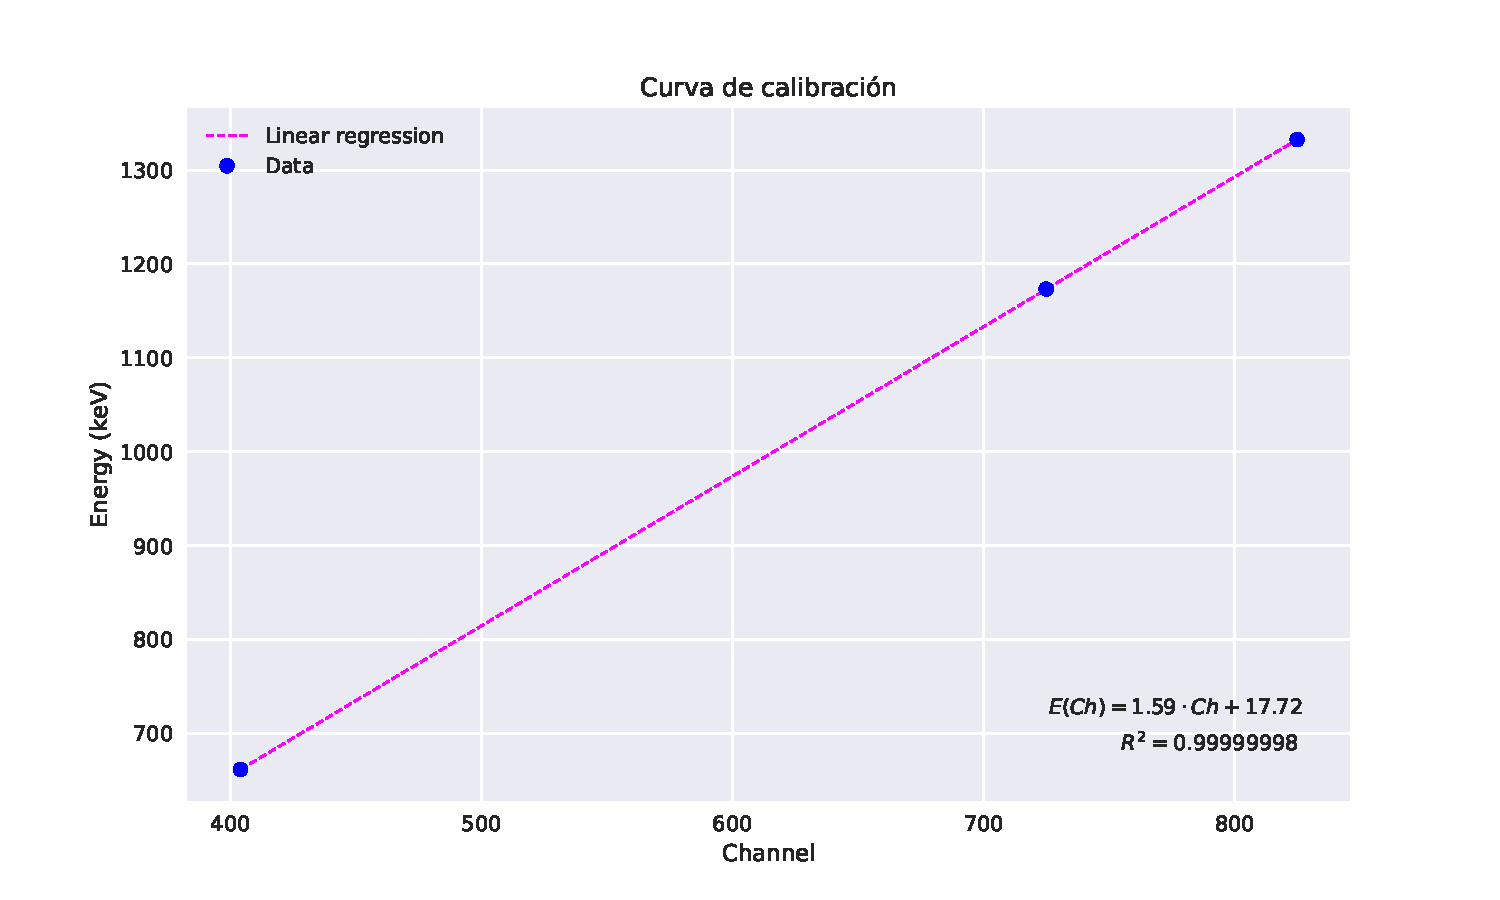
\includegraphics[scale = 0.7]{csi_calibration.pdf}
            \caption{Recta de calibración de energía para el centellador \ch{CsI (Tl)}.}
            \label{fig:csiCalibration}
        \end{figure}

        \subsubsection*{Calibración para el centellador \ch{BGO (BiGeO)}}

        La calibración del centellador \ch{BGO (BiGeO)} se realizó de forma similar a la del centellador \ch{CsI (Tl)} y los datos obtenidos se muestran en la \cref{tab:bgoCalibration}.

        \begin{table}[htb]
            \centering
            \begin{tblr}{
                colspec = {cc},
                hlines,
                rowsep = 4pt,
                row{1} = {font = \bfseries}
            }
                Channel & {Energía \\ (\si{\keV})}  \\
                272     & 661.657 \\             
                502     & 1173.228 \\
                572     & 1332.492
            \end{tblr}
            \caption{Datos de la energía de las gammas de \ch{^{137} Cs} y \ch{^{60} Co} con el centroide de los fotopicos para la calibración del centellador \ch{BGO (BiGeO)}.}
            \label{tab:bgoCalibration}
        \end{table}

        La relación entre la energía y el canal para el centellador \ch{BGO (BiGeO)} que se obtuvo se muestra en la \cref{fig:bgoCalibration} y tiene la forma

        \begin{equation}
            E_{\gamma}(\text{Ch}) = \qty{2.2332 \pm 0.009618}{\keV} \cdot \text{Ch} + \qty{53.8501 \pm 4.4880}{\keV}.
            \label{eq:bgoCalibration}
        \end{equation}

        \begin{figure}[!htb]
            \centering
            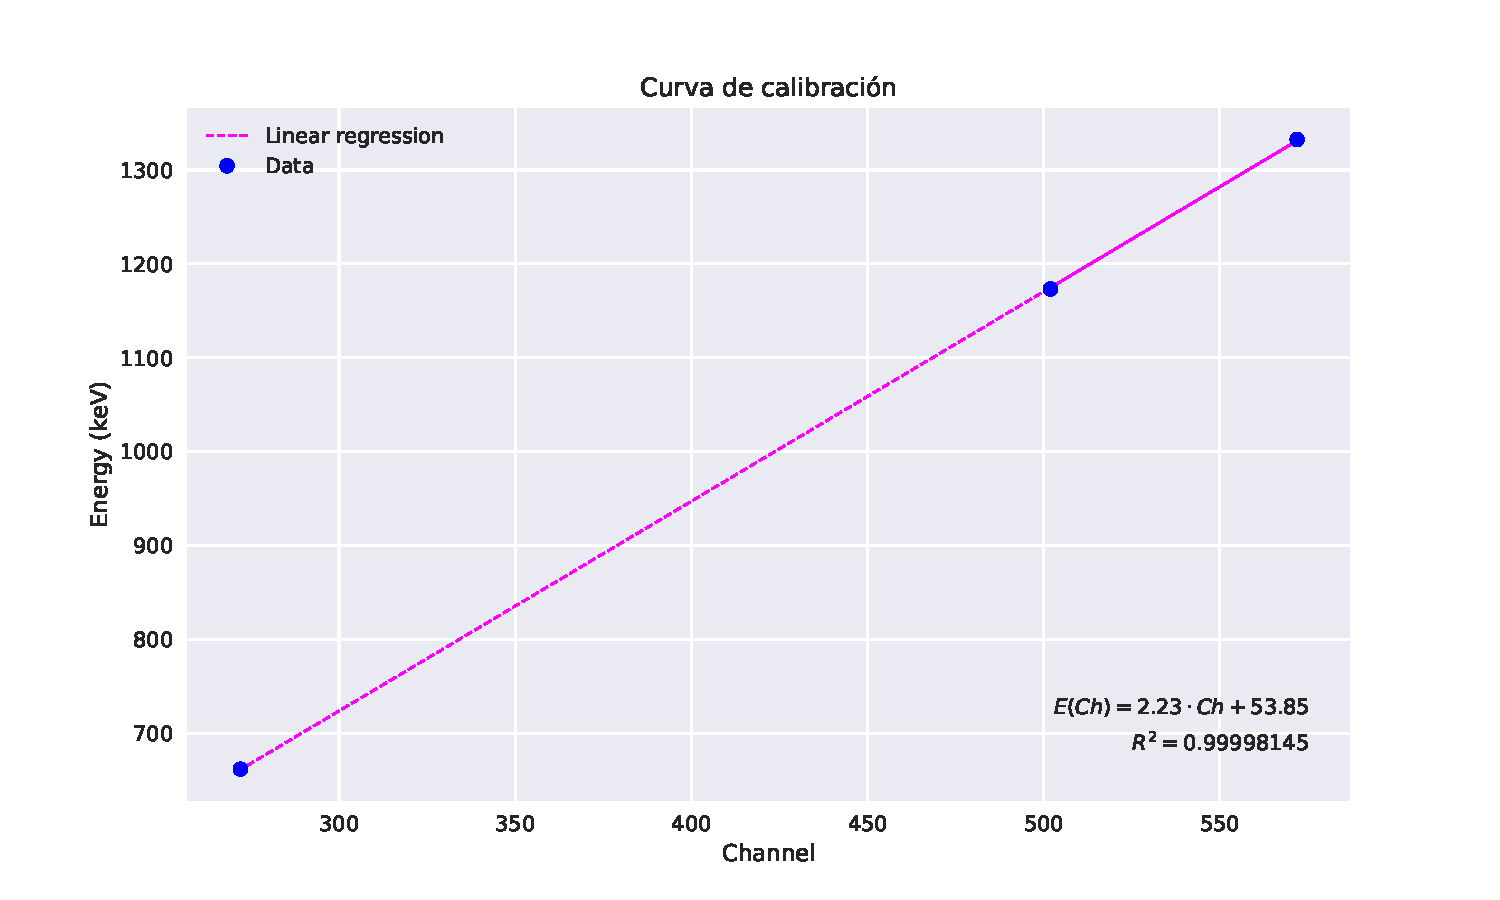
\includegraphics[scale = 0.7]{bgo_calibration.pdf}
            \caption{Recta de calibración de energía para el centellador \ch{BGO (BiGeO)}.}
            \label{fig:bgoCalibration}
        \end{figure}

    \subsection*{Espectros de energía}

    A partir de las \cref{eq:csiCalibration,eq:csiCalibration} se obtuvieron los espectros de Energía contra Número de cuentas para cada uno de los centelladores. Estos espectros se muestran en las \cref{fig:csiCoSpectrum,bgoCsSpectrum}.

    \subsubsection*{Espectro de energía para el centellador \ch{CsI (Tl)}}

    \begin{figure}[!htb]
        \centering
        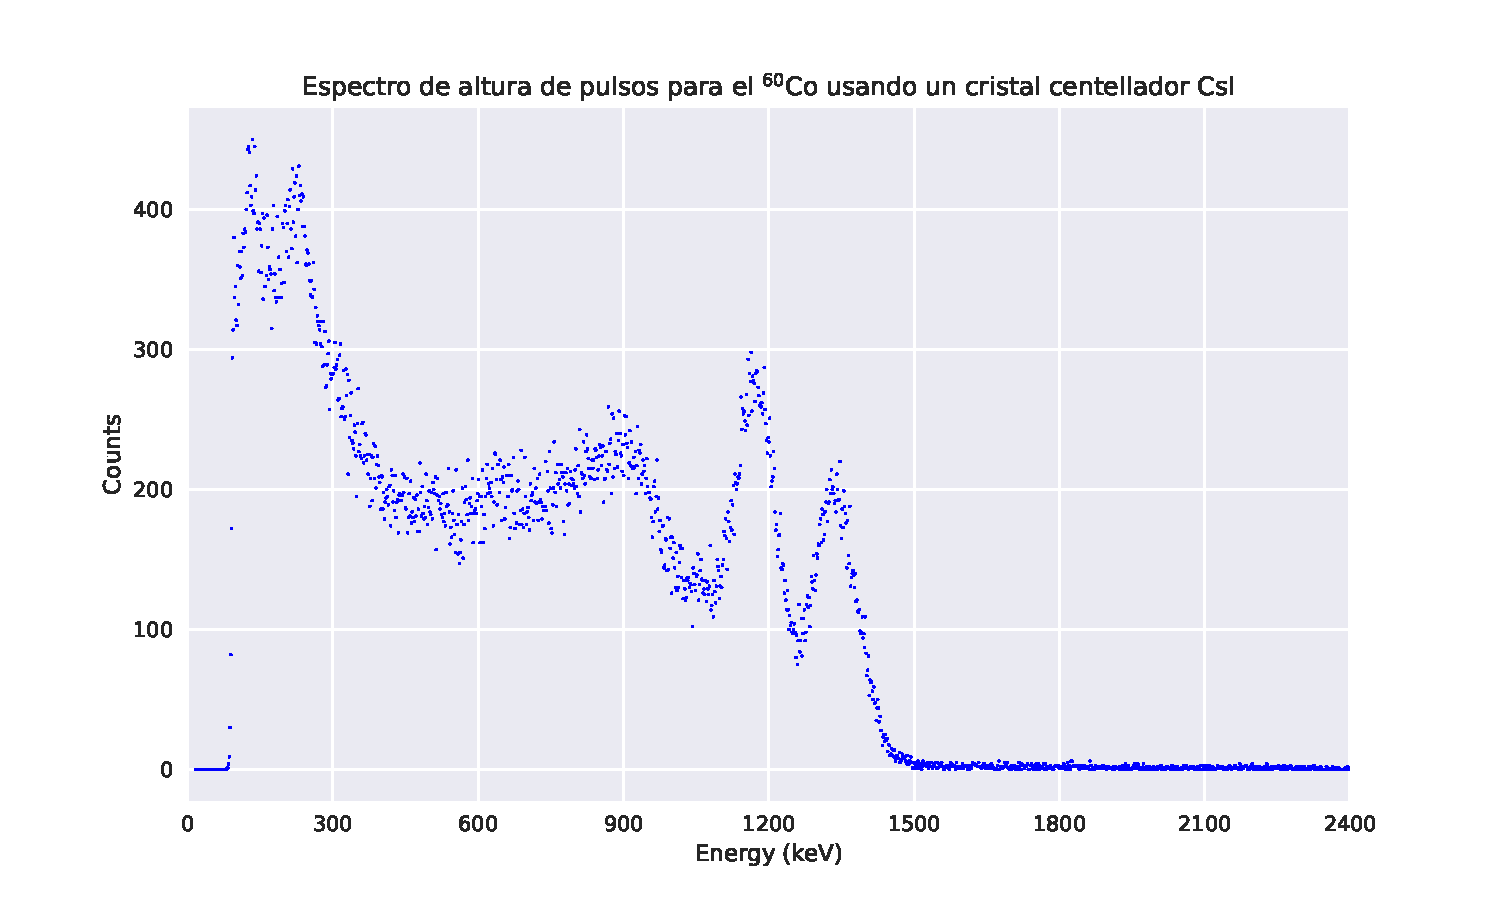
\includegraphics[scale = 0.7]{energy_spectrum_CsICo.pdf}
        \caption{Espectro de energía para el centellador \ch{CsI (Tl)} con la fuente de \ch{^{60} Co}.}
        \label{fig:csiCoSpectrum}
    \end{figure}

    \begin{figure}[!htb]
        \centering
        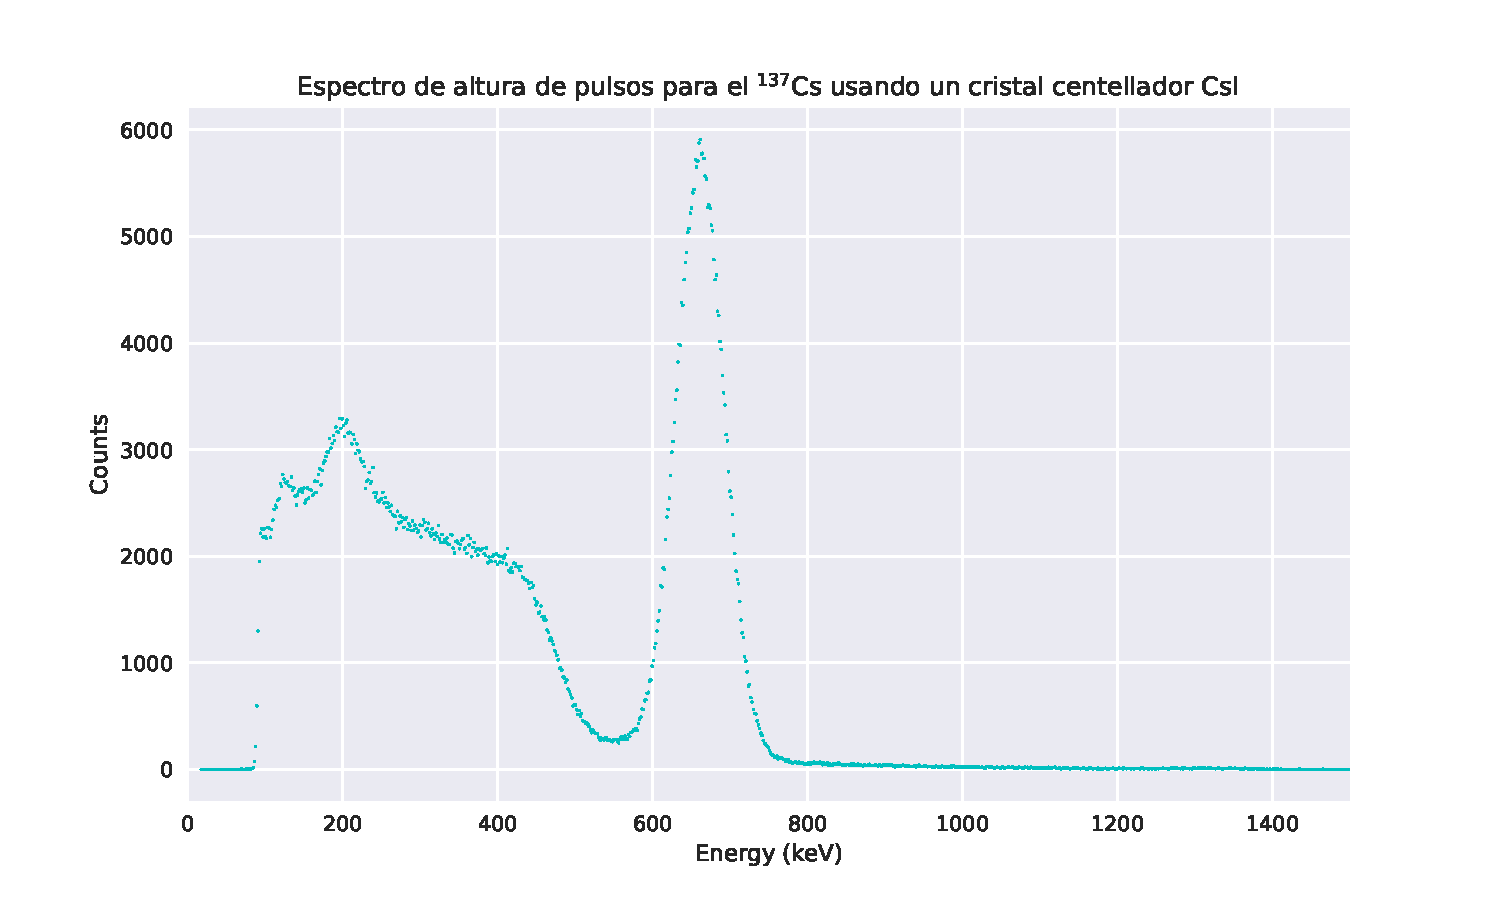
\includegraphics[scale = 0.7]{energy_spectrum_CsICs.pdf}
        \caption{Espectro de energía para el centellador \ch{CsI (Tl)} con la fuente de \ch{^{137} Cs}.}
        \label{fig:csiCsSpectrum}
    \end{figure}

    \subsubsection*{Espectro de energía para el centellador \ch{BGO (BiGeO)}}

    \begin{figure}[!htb]
        \centering
        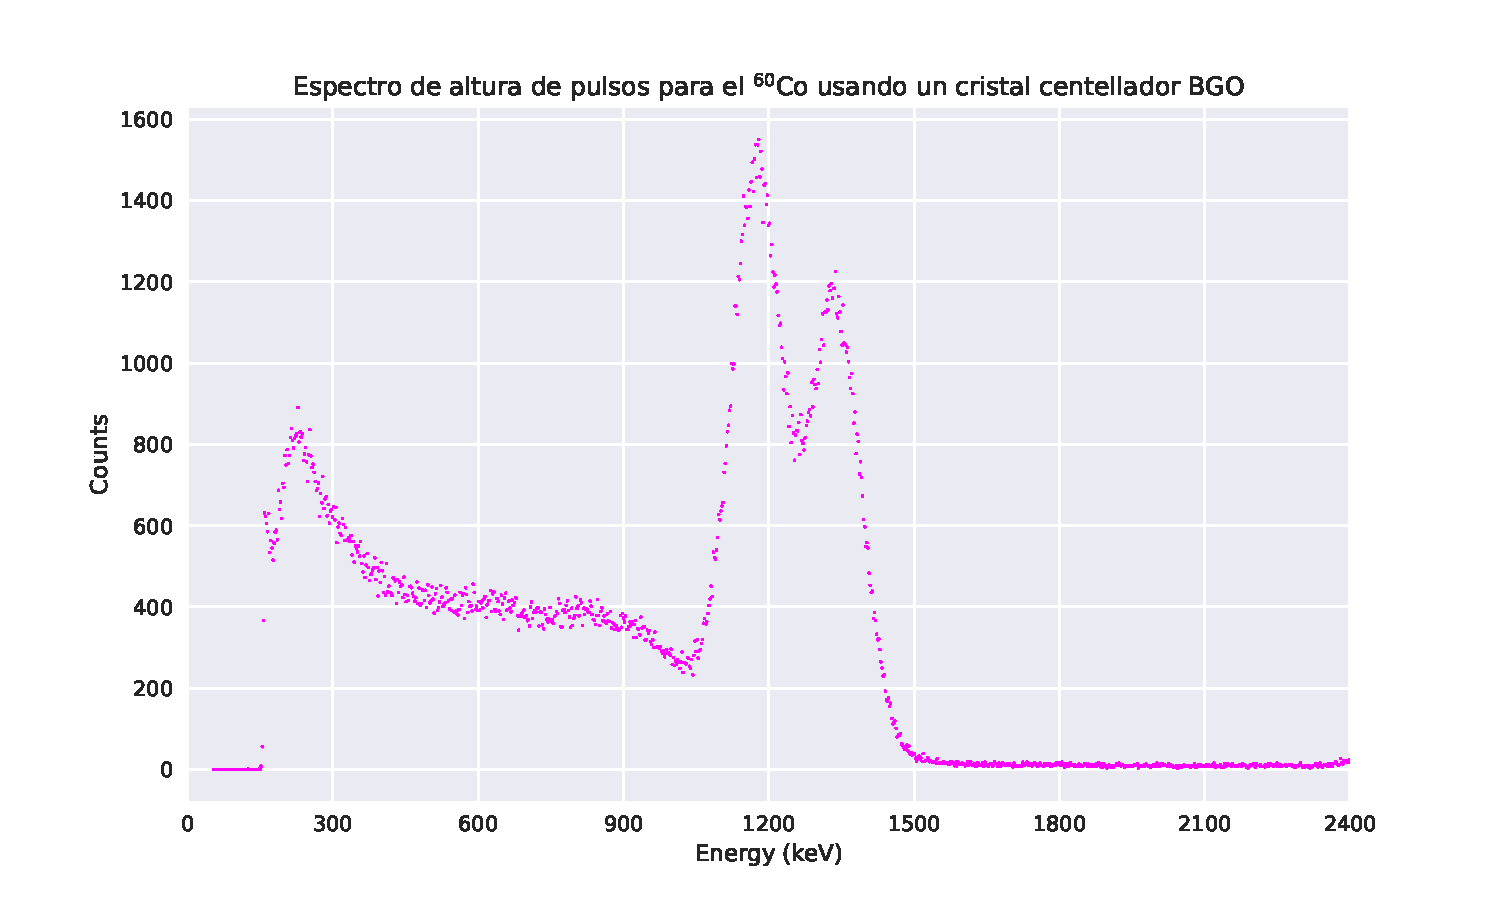
\includegraphics[scale = 0.7]{energy_spectrum_BGOCo.pdf}
        \caption{Espectro de energía para el centellador \ch{BGO (BiGeO)} con la fuente de \ch{^{60} Co}.}
        \label{fig:bgoCoSpectrum}
    \end{figure}

    \begin{figure}[!htb]
        \centering
        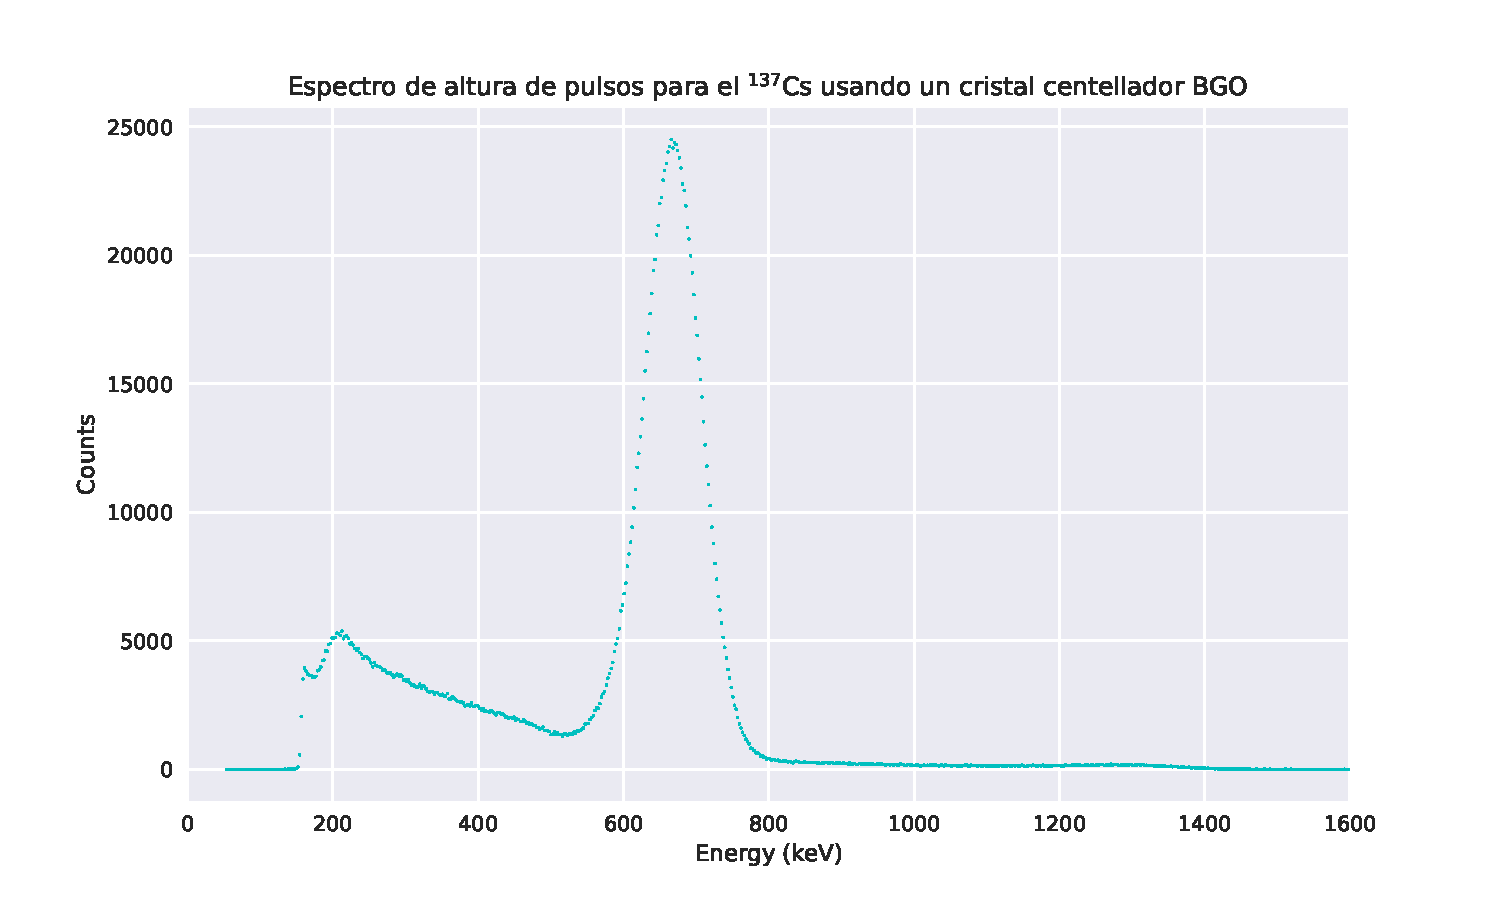
\includegraphics[scale = 0.7]{energy_spectrum_BGOCs.pdf}
        \caption{Espectro de energía para el centellador \ch{BGO (BiGeO)} con la fuente de \ch{^{137} Cs}.}
        \label{fig:bgoCsSpectrum}
    \end{figure}

    \section*{Discusión}
    \kant[1-2]
    
    \section*{Resultados y conclusiones}
    \kant[1]
    
    % \nocite{*} % Show all references    
    % Referencias
    \newpage
    \printbibliography
\end{document}